This section will go through the verification of binary search trees 
and consequently AVL trees in Lean. First I will give some structural definitions for the tree and its properties, 
and then proceed with an explanation of the various proofs completed. 
The textbook released by the University of Pennsylvania \textit{Verified Functional Algorithms} \cite{bst:upenn}
and \textit{Discrete Mathematics with a Computer} \cite{avl:computer} were used as a reference point for some definitions and basic proof statements.

\section{Binary Search Trees}
% \subsection*{Binary Search Trees}
% The first thing to defining an AVL tree is to define a binary search tree. A binary tree 
% definition exists in Lean3 under the inductive type \lstinline{bin_tree}, however the definition is incomplete
% for the purpose of binary search. The \lstinline{bin_tree} constructor \lstinline{leaf} is the only one that includes a 
% definition for a key, and not the constructor dor \lstinline{node}. We want access to subtrees and the key at any given node 
% to define the binary search property, so we create our own definition for a binary tree. This definition can be seen in Figure \ref{lst:btree}.
% The type for the structure is inductive, which is useful for proofs as induction can be performed on any \lstinline{btree}.

% \begin{figure}[!h]
%   \centering
%   \lstinputlisting[language=lean, firstline=3, lastline=5, frame=single]{/Users/sofiakonovalova/Desktop/Thesis/lean-thesis/src/basic.lean}
%   \caption{}
%   \label{lst:btree}
% \end{figure}

% I also define the basic operations for a binary search tree: \lstinline{insert}, \lstinline{bound},
% and \lstinline{lookup}, shown in Figure \ref{lst:basic_ops}. The definition of \lstinline{bound} and \lstinline{lookup} are similar, with bound not serving much reason except for
% using it in later proofs to show that node keys are preserved after other operations.  

% \begin{figure}[!ht]
%   \centering
%   \lstinputlisting[language=lean, firstline=12, lastline=31, frame=single]{/Users/sofiakonovalova/Desktop/Thesis/lean-thesis/src/basic.lean}
%   \caption{}
%   \label{lst:basic_ops}
% \end{figure}

% I also define the binary search property, as shown in Definition \ref{def:bst_property}. For this I created a helper definition, \lstinline{forall_keys}, which 
% defines what exactly it means for all keys in a left or right subtree to be smaller or larger than the root key. This definition is made as abstract as possible, with the 
% greater-than or less-than relation defined as just the \notes{parameter? variable? } \lstinline{p}, which is given a type of \lstinline{nat → nat → Prop}, which is the type definition of the 
% $>$ and $<$ relations in Lean. If the predicate is satisfied in the current node, as well as the left and right subtrees, then the predicate is satisfied in the whole tree. With this definition,
% the formalization of the binary search property is halfway done.

% We call the definition for the binary search property \lstinline{ordered}, as
% it is another name for trees where the property holds. It is also made recursive, as in our inductive \lstinline{btree} definition, we only have direct definition of the left child and the right child, 
% and not the children of those children. There is no guarantee that the grandchildren are ordered, so the definition takes this into account with the recursion: a binary tree can only be ordered if every single subtree 
% is ordered. The complete definition can be seen in Figure \ref{lst:ordered}. 

% \begin{figure}[!ht]
%   \centering
%   \lstinputlisting[language=lean, firstline=35, lastline=38, frame=single]{/Users/sofiakonovalova/Desktop/Thesis/lean-thesis/src/basic.lean}
%   \caption{}
%   \label{lst:forall_keys}
% \end{figure}

% \begin{figure}[!ht]
%   \centering
%   \lstinputlisting[language=lean, firstline=40, lastline=43, frame=single]{/Users/sofiakonovalova/Desktop/Thesis/lean-thesis/src/basic.lean}
%   \caption{}
%   \label{lst:ordered}
% \end{figure}

% \subsection*{Balancing}
% I define the height of a tree as per Definition \ref{def:height} in Figure \ref{lst:height}. \notes{Why is there a +1 in the definition?}

% \begin{figure}[!ht]
%   \centering
%   \lstinputlisting[language=lean, firstline=49, lastline=52, frame=single]{/Users/sofiakonovalova/Desktop/Thesis/lean-thesis/src/basic.lean}
%   \caption{}
%   \label{lst:height}
% \end{figure}

\section{AVL Trees}
\notes{give a small introduction to the section}

\subsection{Binary Search Trees} 
\label{sec:bst}
I begin by defining a binary search tree. A binary tree is a tree data structure where each node can have no more than two children. These two children are 
called the \textit{left child} and the \textit{right child} subtrees. In a binary \textit{search} tree, nodes are placed according to their key. 

Where nodes are placed in a binary search tree is determined by what is often called the \textit{binary search property}.

\begin{definition}[Binary Search Property]
  \label{def:bst_property}
  Given any node N in a binary search tree, all the keys in the left child subtree are smaller than that of N, and all keys in the right child subtree are greater than the 
  key of N.
\end{definition}

This allows for lookup and insertion to be done in \notes{add complexity here} time in the worst case, as at any given node half of the tree is skipped.

\begin{figure}[!h]
  \centering
  \begin{subfigure}{.3\textwidth}
    \centering
    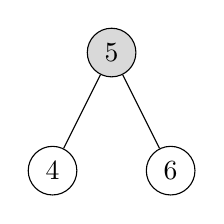
\begin{tikzpicture}
      \node[circle,draw,fill=gray!30](z){5}
      child{ node[circle,draw]{4} }
      child{
        node[circle,draw]{6} child[missing] child[missing] };
    \end{tikzpicture}
    \caption{}
    \label{fig:insert_1}
  \end{subfigure}%
  \begin{subfigure}{.3\textwidth}
    \centering
    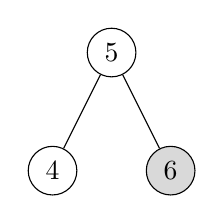
\begin{tikzpicture}
      \node[circle,draw](z){5}
      child{ node[circle, draw]{4} }
      child{
        node[circle,draw,fill=gray!30]{6} child[missing] child[missing] };
    \end{tikzpicture}
    \caption{}
    \label{fig:insert_2}
  \end{subfigure}%
  \begin{subfigure}{.3\textwidth}
    \centering
    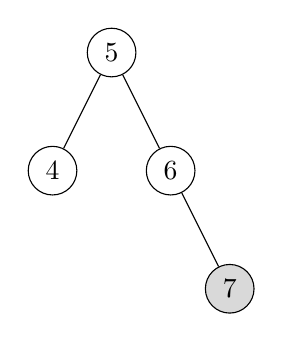
\begin{tikzpicture}
      \node[circle,draw](z){5}
      child{ node[circle, draw]{4} }
      child{
        node[circle,draw]{6} child[missing] child{node[circle,draw,fill=gray!30]{7}} };
    \end{tikzpicture}
    \caption{}
    \label{fig:insert_3}
  \end{subfigure}
  \caption{Insertion operation in a binary search tree.}
  \label{fig:insert_demo}
\end{figure}

Search, insertion and retrieval can be done recursively. Starting at the root node, the input key and the node key are compared: if the input key is smaller,
the operation is done recursively on the left subtree; if the input key is larger, then the operation is done recursively on the right subtree. Figure \ref{fig:insert_demo} shows 
a node with key 7 being inserted into a binary search tree. At \ref{fig:insert_demo}(\ref{sub@fig:insert_1}), the new node is compared to the root. As $7 > 5$, the operation continues at 
the right subtree. At \ref{fig:insert_demo}(\ref{sub@fig:insert_2}) the comparison is done again. As $7 > 6$, the operation continues at the right subtree. Because the node 6 doesn't have any children and $7 > 6$,
a new right child node is created.

\subsection{Balance and rotation}
An AVL tree is based on a binary search tree, with one very important distinction - it is \textit{balanced}. To define what it means for a tree to be balanced, I will first
define what the \textit{height} of a tree is.

\begin{definition}[Tree height]
  \label{def:height}
  The height of a tree is the length of the longest path from the root to a leaf.
\end{definition} 
 
Balance is reliant on this definition - an AVL tree is only balanced when the 
heights of any given left and right child subtrees does not differ by more than one \cite{avl:original}. By keeping balance, the structure ensures that there is a high ratio between the number of 
nodes in the tree and the height. This allows for retrieval and search operations to be done in $O(\log n)$ time in the worst case, with $n$ being the amount of nodes in a tree \cite{avl:computer}.

During the insertion operation, the tree can become imbalanced, which can be mitigated
with either a right rotation or a left rotation. 

\section{Proofs}
This section presents formalizations of some proofs done in relation to AVL trees in Lean. Each section talks about a specific tree operations, and provides some examples of proof statements and informally explains the process of completing the proofs.

% \subsection{BST Operations}
% First, we prove two lemmas related to boundedness and lookup in a tree, since \lstinline{lookup} and \lstinline{bound} are identical for both BSTs and AVL trees.

\begin{lstlisting}
lemma bound_false (k : nat) (t : btree α) :
  bound k t = ff → lookup k t = none := ...

lemma bound_lookup (k : nat) (t : btree α) :
  bound k t → ∃ (v : α), lookup k t = some v := ...
\end{lstlisting}

Both of the proofs were constructed by induction on the tree \lstinline{t}. The lemma \lstinline{bound_false} states that if a key is not bound in a tree, then lookup will not result in any node data being returned. The lemma \lstinline{bound_lookup} states that if a key is bound in a tree, then some data will be returned.

\subsection{Rotation}
With rotations we want to prove that an ordered tree preserves order after a rotation, and that if a tree is imbalanced then a rotation restores its balance. This section will present two proofs on right rotations preserving order and balance.

\subsection*{Order}
\begin{lstlisting}[caption=\empty, label={lst:right_ordered}]
lemma rotate_right_ordered (t : btree α) :
  ordered t → ordered (rotate_right t) := ...
\end{lstlisting}

Listing \ref{lst:right_ordered} shows a formalized lemma statement for right rotations preserving order. The first step with proof statements with rotations is to look at their definitions. The definition for \lstinline{rotate_right} uses the \lstinline{simple_right} and \lstinline{simple_left} definitions, so proofs about them preserving order need to be constructed too.

\begin{lstlisting}[caption=\empty, label={lst:simple_ordered}]
lemma simple_right_ordered (t : btree α) :
  ordered t → ordered (simple_right t) := ...

lemma simple_left_ordered (t : btree α) :
  ordered t → ordered (simple_left t) := ...
\end{lstlisting}

The proof in Listing \ref{lst:right_ordered} were done by case splitting on the tree \lstinline{t}, its right subtree \lstinline{r} and the next subtree \lstinline{lr}, and the simple rotation lemmas were applied throughout when needed. The simple rotation lemmas were also completed by case splitting on left or right subtree depending on the rotation.

The proofs above also require a lemma for transitivity of keys in trees. Assume a tree \lstinline{rr} and \lstinline{rl}, with the former having a left and a right child \lstinline{rll} and \lstinline{rlr}. Also assume two keys \lstinline{rk}, which is the parent node key of \lstinline{rr}, and \lstinline{rlk}, which is the key of \lstinline{rl}.
If \lstinline{rk} is greater than all the keys contained in \lstinline{rll} and \lstinline{rlr}, and \lstinline{rk} is less than the keys in \lstinline{rr}, by transitivity \lstinline{rlk} is less than all the keys in \lstinline{rr}. The lemma for key transitivity is formalized below.

\begin{lstlisting}[caption=\empty]
lemma forall_keys_trans (t : btree α) (p : nat → nat → Prop) 
(z x : nat) (h₁ : p x z) (h₂ : ∀ a b c, p a b → p b c → p a c) :
  forall_keys p z t → forall_keys p x t := ...
\end{lstlisting}

Another lemma had to be made to make constructing proofs with \lstinline{forall_keys} much easier. The current definition for \lstinline{forall_keys} does not take into consideration the relationship of the input key between the left and right children of the tree. The \lstinline{forall_keys_intro} introduction lemma solved this problem.

\begin{lstlisting}[caption=\empty]
lemma forall_keys_intro {l r : btree α} {k x : nat} {v : α} 
  {p : nat → nat → Prop} :
(forall_keys p k l ∧ p k x ∧ forall_keys p k r) 
  → forall_keys p k (node l x v r) := ...
\end{lstlisting}

When applying the introduction lemma, I was able to get the relation of the key between the left and right subtree, and the relation between the input key and the key of the tree, which made applying the transitivity lemma a lot easier.

\subsection*{Balance}

% \subsection{Insertion}
% Proofs about insertion into AVL trees, like the ones for rotation, need to show a preservation of order, keys, and balance restoration.

\subsection{Deletion}
This section details the steps taken to write a proof for deletion preserving order. Similar to proofs about rotations, if we want to prove deletion preserving order, any other definition that \lstinline{delete} uses will have a lemma regarding order as well. Due to the way that \lstinline{ordered} is defined with \lstinline{forall_keys}, lemmas about boundedness are involved as well. Just from writing one lemma about deletion preserving order, we receive lemmas about key preservation as well, that can be used for other proofs. First we follow the steps taken to write the lemmas for order, then lemmas about key preservation are discussed specifically. Lastly, any design changes or additions made during this process are presented.

\subsection*{Order}
 
We begin with the lemma statement for deletion of a key and deletion of a root node preserving order.

\begin{lstlisting}
lemma delete_ordered (t : btree α) (k : nat) :
  ordered t → ordered (delete k t) := ...

lemma del_root_ordered (t : btree α) :
  ordered t → ordered (del_root t) := ...
\end{lstlisting}

The proof for \lstinline{delete_ordered} was constructed with induction on \lstinline{t}, and \lstinline{del_root} was completed with a case split on \lstinline{t}.

The next step is to complete the proof for \lstinline{shrink} preserving order. The proof for shrink needs to contain more information, as we cannot simply state that \lstinline{t} is ordered and therefore \lstinline{sh} is ordered, there needs to be a link between the two trees. Therefore, hypotheses need to contain the result of shrinking the tree, \lstinline{shrink t = some (x, a, sh)}, and that the entire tree is ordered and therefore so is \lstinline{sh}. The proof also concludes that \lstinline{x} is larger than all of the keys in a shrunken tree.

\begin{lstlisting}
lemma shrink_ordered {t sh : btree α} {x : nat} {a : α} :
  ordered t ∧ shrink t = some (x, a, sh) →
    ordered sh ∧ forall_keys gt x sh := ...
\end{lstlisting}

This lemma, could have been be split into two separate lemmas with one concluding that \lstinline{sh} is ordered and that \lstinline{x} is greater than all keys in \lstinline{sh}. If the lemma was to be separated into two, the induction hypotheses would not be strong enough to complete the proofs.

The proof for \lstinline{shrink_ordered} was done by induction on the tree generalizing \lstinline{x}, \lstinline{a} and \lstinline{sh}.

In the inductive step, if the left subtree is larger than the height of \lstinline{sh + 1}, then \lstinline{sh = rotate_right (node l k v sh_1)}, where \lstinline{sh_1} is from \lstinline{shrink r = (x_1, a_1, sh_1)}. This case can be resolved with the lemma \lstinline{rotate_right_keys} to show that keys are preserved after a rotation. Then we need to show that all the keys in \lstinline{sh} come from the original tree, which is done by applying the lemma \lstinline{shrink_keys}.

\begin{lstlisting}
lemma shrink_keys {t sh : btree α} {x : nat} {a : α} :
  ordered t ∧ shrink t = some (x, a, sh) → 
    bound x t ∧ (∀ k', bound k' t → bound k' sh) := ...
\end{lstlisting}

We know that \lstinline{x_1} is larger than all the keys in \lstinline{sh_1}. Since \lstinline{(node l k v sh_1)} is ordered, then it must be the case that \lstinline{k} is smaller than all the keys in \lstinline{sh_1}, and therefore \lstinline{x > k} and \lstinline{x} is greater than all the keys in \lstinline{l}. This is formalized using the auxiliary lemma \lstinline{forall_shrink}.

\begin{lstlisting}
lemma forall_shrink {t sh : btree α} {k x : nat} {a : α} 
{p : nat → nat → Prop} :
  forall_keys p k t ∧ shrink t = some (x, a, sh) → 
    forall_keys p k sh ∧ p k x :=
\end{lstlisting}

As \lstinline{shrink_keys} would have to be applied to \lstinline{shrink_ordered}, the original \lstinline{forall_keys} definitions had to be rewritten. The original definition, \lstinline{forall_keys_unfolded}, was a recursive one that looked at the relation of the key to the left and right tree, and with the current node key. It presents nothing about the key being bound in the tree it has a relation with, even though it is a safe assumption to make. In order to use \lstinline{shrink_keys}, we need a definition of \lstinline{forall_keys} that includes the assumption of boundedness, but still compares the input key to keys in a tree. The result was the current definition of \lstinline{forall_keys}.

\begin{lstlisting}
def forall_keys_unfolded (p : nat → nat → Prop) : nat → btree α → Prop
| x btree.empty := tt
| x (btree.node l k a r) :=
  forall_keys_unfolded x l ∧ (p x k) ∧ forall_keys_unfolded x r
\end{lstlisting}

After the new definition was written, a characterization lemma was needed in order to be able to work with the two different definitions, because we don't necessarily need the hypothesis that the keys compared are bound in the tree in all the proof constructions, or even in the entire proof construction.

The characterization lemma being a bi-implication allows for the lemma to be applied to any hypothesis containing a \lstinline{forall_keys}, to extract information about the subtrees separately and the relationship between \lstinline{k} and \lstinline{x}. This made proof constructions with \lstinline{forall_keys} significantly easier, as there was an alternative way to unfold \lstinline{forall_keys}, instead of unfolding it in terms of \lstinline{bound} like in the definition. 

\begin{lstlisting}
lemma forall_keys_ch {l r : btree α} {k x : nat} {v : α} 
{p : nat → nat → Prop} :
  (forall_keys p k l ∧ p k x ∧ forall_keys p k r) ↔ 
    forall_keys p k (node l x v r) :=
\end{lstlisting}

\subsection*{Views}

During most proof constructions presented in this section, I simplified definitions to extract information, or create case splits. With \lstinline{shrink}, this process would be long and would clutter the proof. There needed to be a way to split the result of \lstinline{shrink} into the tree possible cases that can come out of shrinking a tree with one action, reducing any unnecessary writing. The same problem arose with \lstinline{del_node}. To solve these problems we define two views for \lstinline{shrink}\footnote{This approach was suggested by Jannis Limperg} and \lstinline{del_node}. The \lstinline{shrink_view} is shown below.

\begin{lstlisting}
inductive shrink_view {α} : btree α → option (nat × α × btree α) → Sort*
| empty : shrink_view empty none
| nonempty_empty : ∀ {l k v r},
  shrink r = none →
  shrink_view (node l k v r) (some (k, v, l))
| nonempty_nonempty₁ : ∀ {l k v r x a sh out},
  shrink r = some (x, a, sh) →
  height l > height sh + 1 →
  out = some (x, a, rotate_right (btree.node l k v sh)) →
  shrink_view (node l k v r) out
| nonempty_nonempty₂ : ∀ {l k v r x a sh},
  shrink r = some (x, a, sh) →
  height l ≤ height sh + 1 →
  shrink_view (node l k v r) (some (x, a, node l k v sh))
\end{lstlisting}

The views have a constructor for each possible result of \lstinline{shrink} or \lstinline{del_node}. In the case where rotations are made, an adjustment had to be made in the form of the assumption \lstinline{out}. This was done because inductive types in Lean do not accept other function calls in the type constructor.

In order to use the views, auxiliary lemmas were written to apply a normal \lstinline{shrink} or \lstinline{del_node} and get the three case splits. The lemma for \lstinline{shrink_view} is shown below. The proof for \lstinline{del_node} is almost identical.

\begin{lstlisting}
lemma shrink_shrink_view (t : btree α) : 
  shrink_view t (shrink t) := ...
\end{lstlisting}

Applying the lemma would result in three cases in the inductive step of \lstinline{shrink_ordered}, which matches the three cases from the definition -- one for the right subtree being empty, leading to \lstinline{shrink r = none}, another one where \lstinline{shrink r = some (x, a, rotate_right(l k v sh))}, and another one where \lstinline{shrink r = some (x, a, node l k v sh)}. This allowed to complete the proofs without creating additional case splits, cluttering the proof construction.